\section{Transformer Design}

With given parameters, a transformer is designed and optimized. MATLAB code for this operation is present in this section of the report.\\


% This LaTeX was auto-generated from MATLAB code.
% To make changes, update the MATLAB code and republish this document.

\documentclass{article}
\usepackage{graphicx}
\usepackage{color}

\sloppy
\definecolor{lightgray}{gray}{0.5}
\setlength{\parindent}{0pt}

\begin{document}

    
    
\section*{TRANSFORMER DESIGN}

\begin{par}
EE564 Project\#1 Q2 by G. Hande Bayazit
\end{par} \vspace{1em}

\subsection*{Contents}

\begin{itemize}
\setlength{\itemsep}{-1ex}
   \item Parameters
   \item Sizing
   \item Conclusion
\end{itemize}


\subsection*{Parameters}

\begin{verbatim}
B_op=1.5; %T
mu=1.83/800;
f=50; %Hz
P1= 500e3; %W
V1=34500; %V
V2=25000; %V
I1=P1/V1; %A
J=4; %A/mm^2
a_cable=I1/J; %mm^2
fprintf('Cable area should be around %d mm^2.\n',a_cable);

% This value is close to AWG11 size.

a_cable=4.1684; %mm^2
dia_cable=2.30378; %mm
res_cable=4.1328; %Ohms/km
\end{verbatim}

        \color{lightgray} \begin{verbatim}Cable area should be around 3.623188e+00 mm^2.
\end{verbatim} \color{black}
    

\subsection*{Sizing}

\begin{verbatim}
% Recalling the equation: V_ind=2*pi/sqrt(2)*f*B*A*N
% A*N is constant and they are dependent on each other. Optimum values of
% them will be found with an optimization parameter "k".

ff=0.5; %fill factor
dens_steel=7650; %kg/m^3
dens_copper=8940; %kg/m^3
core_loss_dens=0.77; %W/kg
price_steel=3; %$/kg
price_copper=7; %$/kg

i=1;
for k=5:15

    N1(:,i)=69*k;
    N2(:,i)=50*k;
    A(:,i)=V2*sqrt(2)/(2*pi*f*B_op*N1(:,i)); %m^2

    % Window area

    x1(:,i)=dia_cable*23/ff/1000; %m
    x2(:,i)=dia_cable*3*k/ff/1000; %m
    x3(:,i)=ceil(sqrt(A(:,i)*10000))/100; %m

    w1(:,i)=x1(:,i);
    w2(:,i)=2*x2(:,i)+0.03;

%     fprintf('Window area is %d m^2.\n',w1(:,i)*w2(:,i));

    % Overall dimensions

    e1(:,i)=w1(:,i)+2*x3(:,i);
    e2(:,i)=w2(:,i)+2*x3(:,i);

%     fprintf('Dimensions of the transformer is %d x %d x %d m.\n',e1(:,i),e2(:,i),x3(:,i));

    vol(:,i)=(e1(:,i)*e2(:,i)-w1(:,i)*w2(:,i))*x3(:,i);

    m_steel(:,i)=dens_steel*vol(:,i);

%     fprintf('Steel mass is %d kg.\n',m_steel(:,i));

    core_loss(:,i)=core_loss_dens*m_steel(:,i);

%     fprintf('Core loss is %d Watts.\n',core_loss(:,i));

    % Cable length

    mean_length(:,i)=2*(x2(:,i)/2+x3(:,i))+pi*x3(:,i)*sqrt(2); %m
    l1(:,i)=mean_length(:,i)*N1(:,i);
    l2(:,i)=mean_length(:,i)*N2(:,i);

    r1(:,i)=l1(:,i)*res_cable/1000; %Ohms
    r2(:,i)=r1(:,i)*(N2(:,i)/N1(:,i))^2; %Ohms

    vol_copper(:,i)=2*l1(:,i)*a_cable/1000000; %m^3
    m_copper(:,i)=vol_copper(:,i)*dens_copper; %kg

%     fprintf('Copper mass is %d kg.\n',m_copper(:,i));

    copper_loss(:,i)=I1^2*r1(:,i)*2; %W

%     fprintf('Copper loss is %d Watts.\n',copper_loss(:,i));

    % Inductances

    % Assuming L1 and L2 are 0.02 pu;

    ind1=V1^2/(P1*2*pi*f)*0.02; %H
    ind2=ind1*(N2/N1)^2; %H

    Leff(:,i)=2*(w1(:,i)+w2(:,i)+2*x3(:,i)); %m

    ind_m(:,i)=N1(:,i).^2*mu*A(:,i)/Leff(:,i); %H

    % Efficiency

    eff(:,i)=P1/(P1+core_loss(:,i)+copper_loss(:,i))*100; %percent

    % Cost

    cost(:,i)=price_copper*m_copper(:,i)+price_steel*m_steel(:,i); %$

    %Unit price of electricity: 0.4482 TL = 0.1125 USD

    lost_power(:,i)=P1*(100-eff(:,i))/1000; %kW

    lost_energy(:,i)=lost_power(:,i)*24*365*20*0.1125; %$

    cost_actual(:,i)=cost(:,i)+lost_energy(:,i); %$


    i=i+1;
end
\end{verbatim}


\subsection*{Conclusion}

\begin{verbatim}
% Considering the optimizaton results, optimum case for the design seems to
% be i=6, k=10. Transformer parameters are as follows:

k=10;
i=6;

    N1(:,i)=69*k;
    N2(:,i)=50*k;
    A(:,i)=V2*sqrt(2)/(2*pi*f*B_op*N1(:,i)); %m^2



    % Window area

    x1(:,i)=dia_cable*23/ff/1000; %m
    x2(:,i)=dia_cable*3*k/ff/1000; %m
    x3(:,i)=ceil(sqrt(A(:,i)*10000))/100; %m

    w1(:,i)=x1(:,i);
    w2(:,i)=2*x2(:,i)+0.03;


    % Overall dimensions

    e1(:,i)=w1(:,i)+2*x3(:,i);
    e2(:,i)=w2(:,i)+2*x3(:,i);

    vol(:,i)=(e1(:,i)*e2(:,i)-w1(:,i)*w2(:,i))*x3(:,i);

    m_steel(:,i)=dens_steel*vol(:,i);

    core_loss(:,i)=core_loss_dens*m_steel(:,i);

    % Cable length

    mean_length(:,i)=2*(x2(:,i)/2+x3(:,i))+pi*x3(:,i)*sqrt(2); %m
    l1(:,i)=mean_length(:,i)*N1(:,i);
    l2(:,i)=mean_length(:,i)*N2(:,i);

    r1(:,i)=l1(:,i)*res_cable/1000; %Ohms
    r2(:,i)=r1(:,i)*(N2(:,i)/N1(:,i))^2; %Ohms

    vol_copper(:,i)=2*l1(:,i)*a_cable/1000000; %m^3
    m_copper(:,i)=vol_copper(:,i)*dens_copper; %kg

    copper_loss(:,i)=I1^2*r1(:,i)*2; %W

    % Inductances

    % Assuming L1 and L2 are 0.02 pu;

    ind1=V1^2/(P1*2*pi*f)*0.02; %H
    ind2=ind1*(N2/N1)^2; %H

    Leff(:,i)=2*(w1(:,i)+w2(:,i)+2*x3(:,i)); %m

    ind_m(:,i)=N1(:,i).^2*mu*A(:,i)/Leff(:,i); %H

    % Efficiency

    eff(:,i)=P1/(P1+core_loss(:,i)+copper_loss(:,i))*100; %percent

    % Cost

    cost(:,i)=price_copper*m_copper(:,i)+price_steel*m_steel(:,i); %$


    %Unit price of electricity: 0.4482 TL = 0.1125 USD

    lost_power(:,i)=P1*(100-eff(:,i))/1000; %kW

    lost_energy(:,i)=lost_power(:,i)*24*365*20*0.1125; %$

    cost_actual(:,i)=cost(:,i)+lost_energy(:,i); %$

    fprintf('Turns ratio is %d : %d. \n',N1(:,i),N2(:,i));

    fprintf('Window area is %d m^2.\n',w1(:,i)*w2(:,i));

    fprintf('Dimensions of the transformer is %d x %d x %d m.\n',e1(:,i),e2(:,i),x3(:,i));

    fprintf('Steel mass is %d kg.\n',m_steel(:,i));

    fprintf('Core loss is %d Watts.\n',core_loss(:,i));

    fprintf('R1= %d Ohms, R2= %d Ohms. \n',r1(:,i),r2(:,i));

    fprintf('Copper mass is %d kg.\n',m_copper(:,i));

    fprintf('Copper loss is %d Watts.\n',copper_loss(:,i));

    fprintf('L1= %d H, L2= %d H, Lm= %d H. \n',ind1,ind2,ind_m(:,i));

    fprintf('Efficiency is %d percent. \n',eff(:,i));

    fprintf('Material cost is %d USD. Lost money in 20 years is %d USD. \n',cost(:,i),cost_actual(:,i));
\end{verbatim}

        \color{lightgray} \begin{verbatim}Turns ratio is 690 : 500. 
Window area is 3.247608e-02 m^2.
Dimensions of the transformer is 7.659739e-01 x 9.664536e-01 x 3.300000e-01 m.
Steel mass is 1.786846e+03 kg.
Core loss is 1.375872e+03 Watts.
R1= 6.457173e+00 Ohms, R2= 3.390660e+00 Ohms. 
Copper mass is 1.164488e+02 kg.
Copper loss is 2.712528e+03 Watts.
L1= 1.515473e-01 H, L2= 7.957747e-02 H, Lm= 5.521107e+01 H. 
Efficiency is 9.918895e+01 percent. 
Material cost is 6.175681e+03 USD. Lost money in 20 years is 7.999056e+06 USD. 
\end{verbatim} \color{black}
    


\end{document}
    


Here, for the design of the transformer, the main objective is to find an optimum point where $P_{core}=P_{copper}$, since this is the case where efficiency is maximum.\\

These two variables are dependent on each other, since induced voltage in the tranformer includes a constant term "N*A". This implies that number of turns of the transformer should be inversely proportional to the cross-section area of the core, which are actually the parameters that determines core and copper losses.\\

A graph that shows the relationship of core loss, copper loss and efficiency is given in Figure \ref{cce}. The optimum point is chosen as the point where efficiency is maximum. However at this point, core loss and copper loss are not exactly equal to each other. This discrepancy is caused by (wire mean length) assumptions made in calculation of copper loss.

\begin{figure}[H]
\hspace{1.5cm}
\centering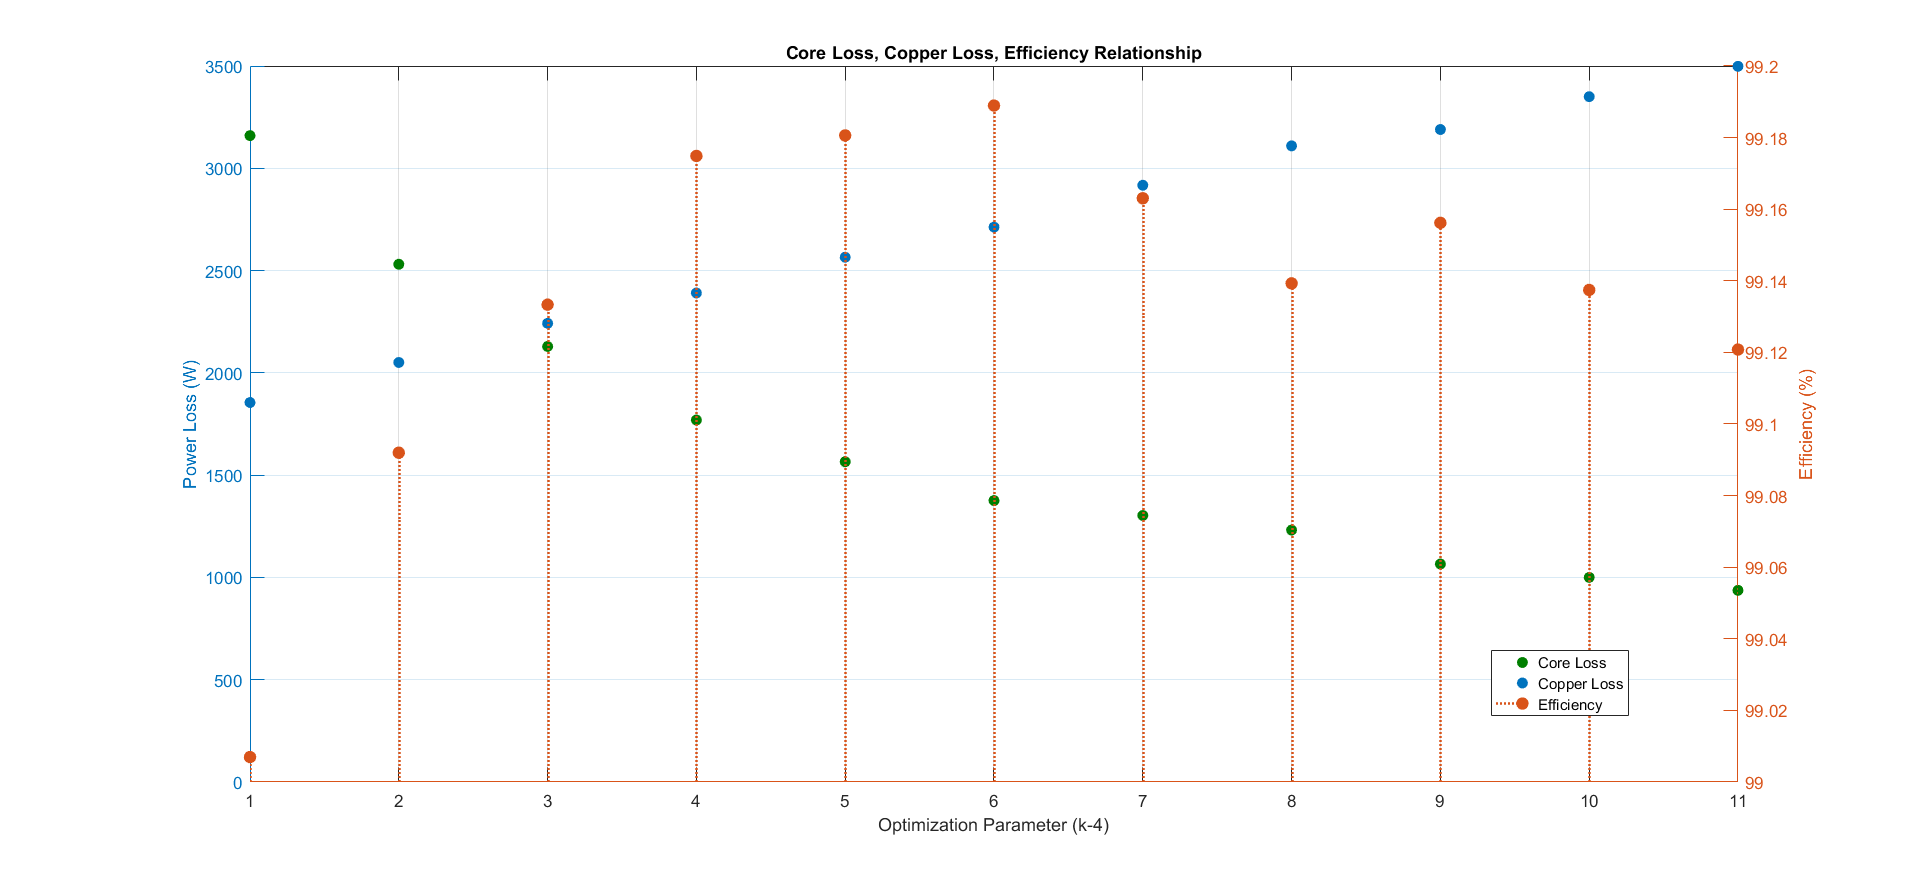
\includegraphics[width=5.5in]{core_copper_eff.PNG}\\
\caption{Relationship Between Core Loss, Copper Loss and Efficiency}
\label{cce}
\end{figure}

Another concern in design of a transformer is obviously the price. What is important is not only the material price of the transformer, but also the money lost due to power lost while the transformer operates. Therefore cost should be considered in both cases. A graph showing this cost analysis is provided in Figure \ref{cost}. Here, the most optimum case is also same as the previous one, since its efficiency is the highest.

\begin{figure}[H]
\hspace{1.5cm}
\centering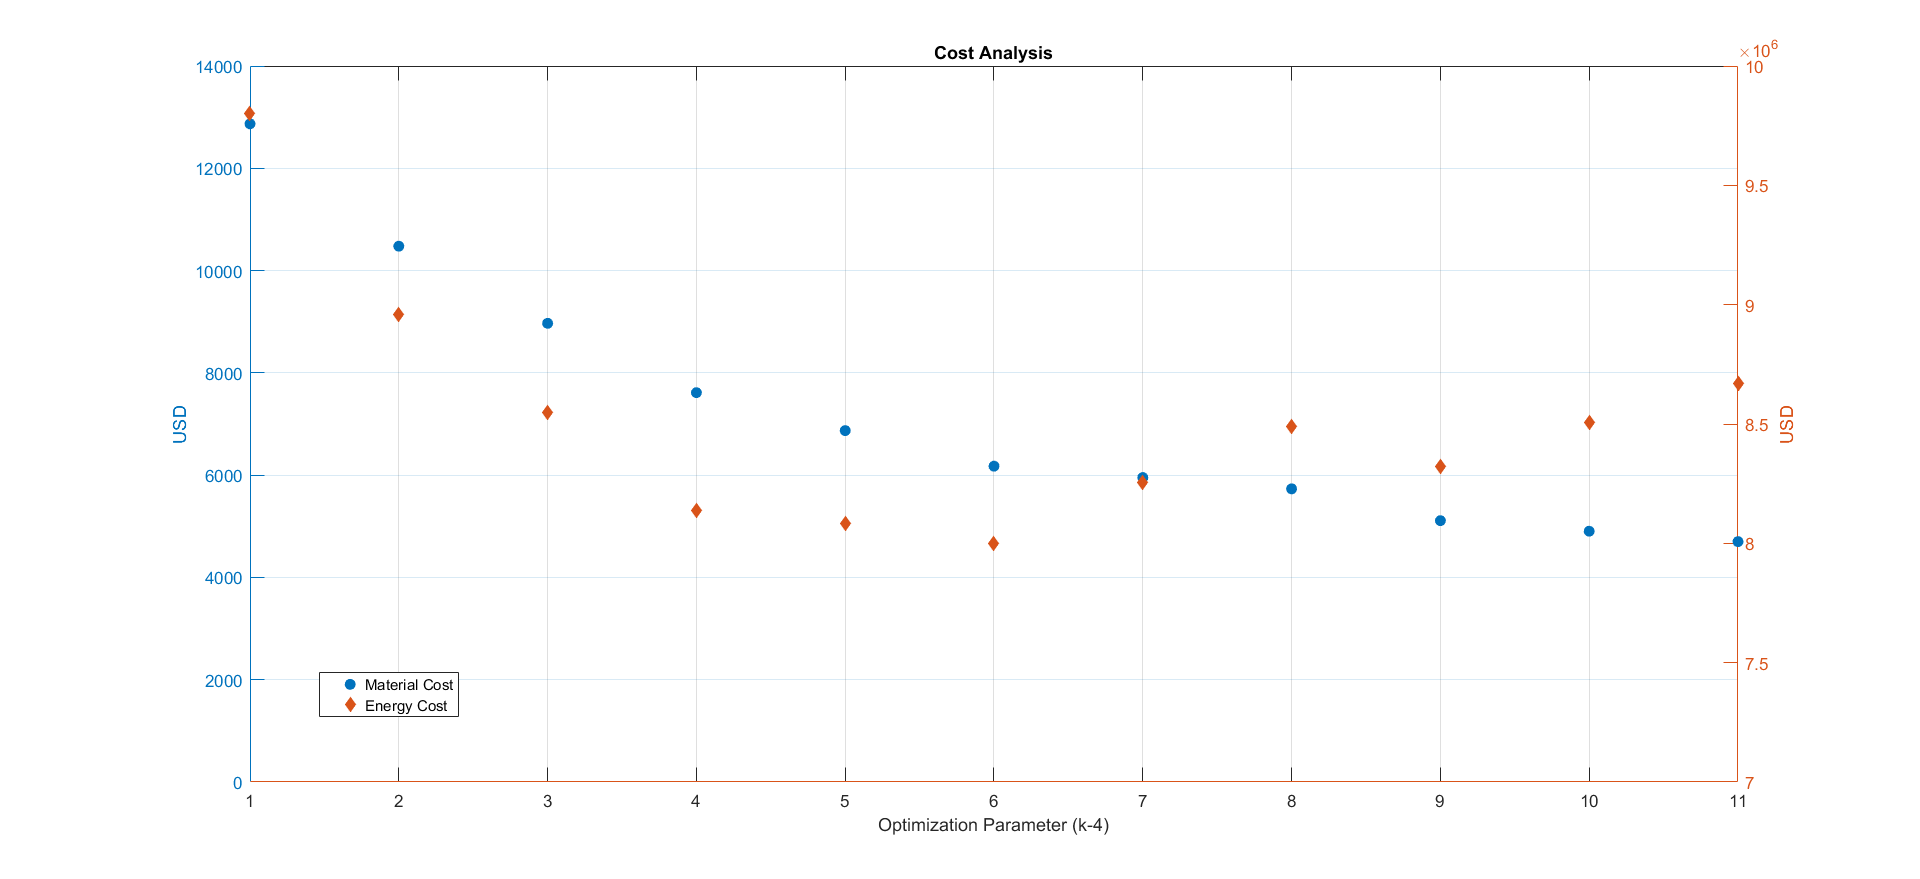
\includegraphics[width=5.5in]{cost.PNG}\\
\caption{Cost Analysis}
\label{cost}
\end{figure} 

Different lamination types also effects the specifications of the transformer. As can be seen in Figure \ref{steel}, core losses increase with increasing lamination thickness. This would have a significant effect on efficiency.\\

In this design, first lamination type (C120-23) is considered. 

\begin{figure}[H]
\hspace{1.5cm}
\centering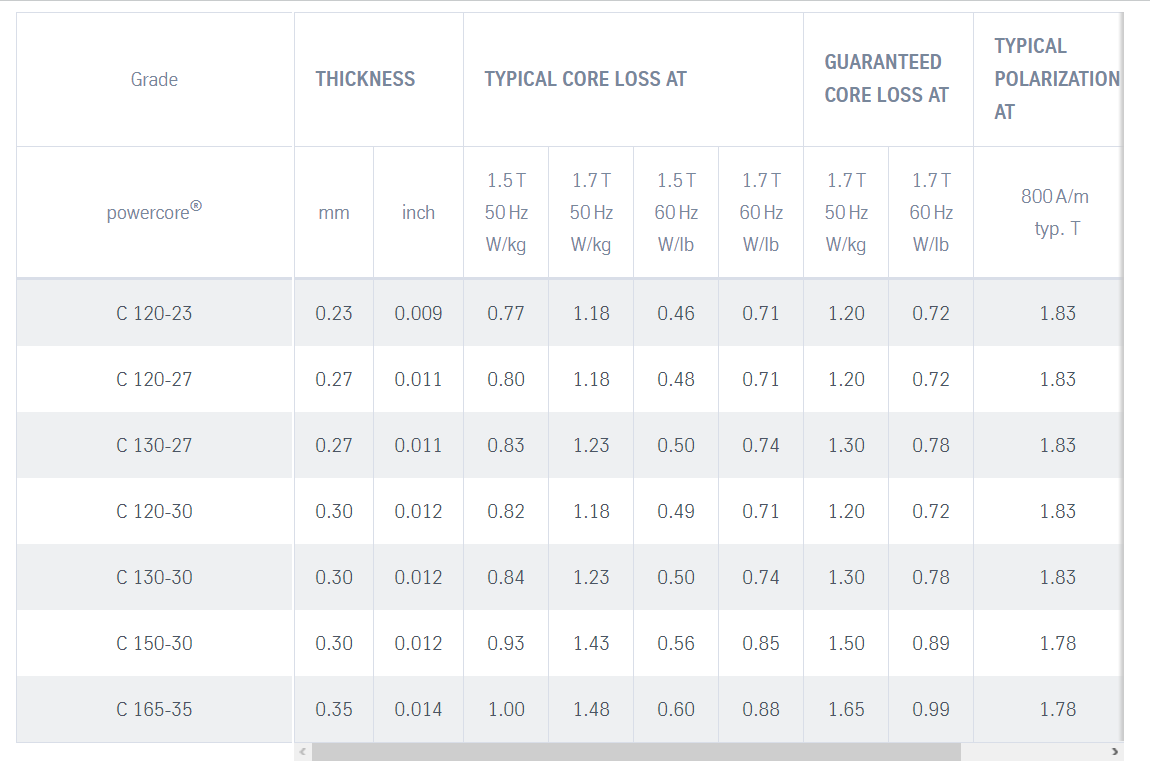
\includegraphics[width=4.5in]{steel_prop.PNG}\\
\caption{Properties of Steel Laminations}
\label{steel}
\end{figure} 
